Since our complete meta-model~\cite{ecore-complete} is of considerable size, we will in this section explain it using a collection of smaller Ecore diagrams. We also explain the key concepts behind the definition of policies.
 
By using Eclipse~\cite{eclipse}, EMF and Xtext we built a domain specific language that is rich enough to express the policies discovered in the analysis. We developed a grammar that is based on our programming experience, and believed to have a consistent forthcoming syntax and conceptual constructs (see \nameref{app:PedslXtext}). Finally, we used our Policy Engine DSL editor to specify buildings and write examples of policies learned from the interviews. The full DSL implementation based on two of the interviews,  Br\"{u}el \& Kj\ae r (see \nameref{app:bogk}) and  K\o benhavns Tekniske Skole (see \nameref{app:kts}). The referenced DSL figures are all cropped from screendumps of actual, running Eclipse instances.

\subsection{Meta-Models}

The following core packages, differentiated in separate Ecore Diagrams can be viewed fully in ~\cite{ecore-complete} as a single meta-model. In the subsections below, we show images and explain the build up of the core package as it is in our model. 

\subsubsection{Building definition}
In order to specify the building(s) with all their floors and rooms, the core classes has been included in fig. \ref{fig:ecore-building-definition}. They all inherit from NamedElement, making it possible to give them a name than can be used for later referencing.
\begin{figure}[h]
  \centering 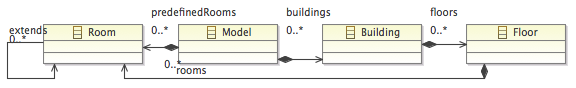
\includegraphics[scale=.5]{ecore-building-definition.png}  
	\caption{The meta-model related to the \textit{building definition}. The inherited class NamedElement has been omitted.}
	\label{fig:ecore-building-definition}
\end{figure}

\subsubsection{Sensors and Actuators}
In our meta-model, the sensors and actuators used are from the combined analysis of the interviews mentioned in the section above. In the meta-model, we have a total of 9 sensor classes and 6 actuator classes. Sensor and Actuator classes inherit from NamedElement, which gives declared elements a name that later can be referenced in other parts of our DSL. If new types are needed, they should be defined in the meta-model.

\begin{figure}[h]
	\centering
    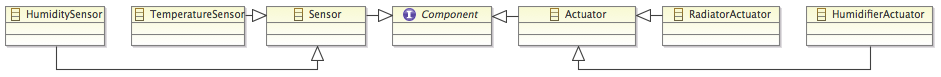
\includegraphics[scale=.7]{ecore-sensors-actuators.png} 
	\caption{A fragment of the \textit{sensor} and \textit{actuator} meta-model hierarchy.}
	\label{fig:ecore-sensors-actuators}
\end{figure}


\subsubsection{Expression Language}
After the analysis of the interviews we concluded that the needed expression language did not need to be very advanced. We needed boolean variables (\textit{states}) and if-statements with two different types of conditions; the normal if-statement --- which operates on sensor types and state instances -- and another that operates on a timer (see fig.\ref{fig:dsl-conditionalexpression}). In the body of the if-statement, we can use an expression to reset timers, and set actuator values using instances in specific rooms as shown in the DSL example in fig.\ref{fig:dsl-policy-definition}. The core classes are all included in fig.\ref{fig:ecore-expression-language} below.

\begin{figure}[h]
  \centering
    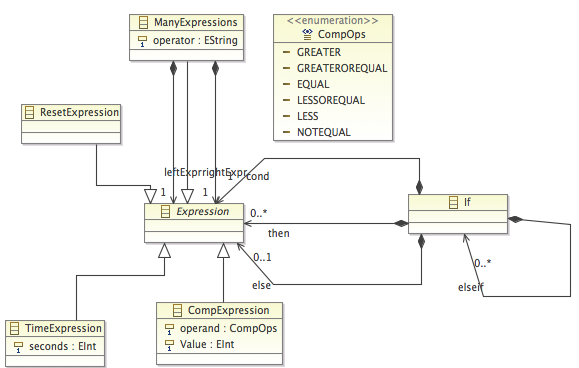
\includegraphics[scale=.5]{ecore-expression-language.png} 
	\caption{The meta-model related to the \textit{expression language}. The inherited class NamedElement has been omitted.}
	\label{fig:ecore-expression-language}
\end{figure}

\subsubsection{Policy definition}
The policy definition meta-model can be inspected in fig. \ref{fig:ecore-policy-definition}. To define a policy, we make use of actuator types, sensor types and room instances (via \texttt{usesRooms}). The implementation of the policy is enhanced by the use of the statements; \textit{if}, \textit{state} and \textit{timer}. The if-statement uses the expression language to define it's behavior. \textit{Schedule} can be defined so that policies are temporally constrained --- as can be inspected in fig.~\ref{fig:room-types}. All policy definition core classes are displayed in fig.\ref{fig:ecore-policy-definition}.
\begin{figure}[h]
  \centering
    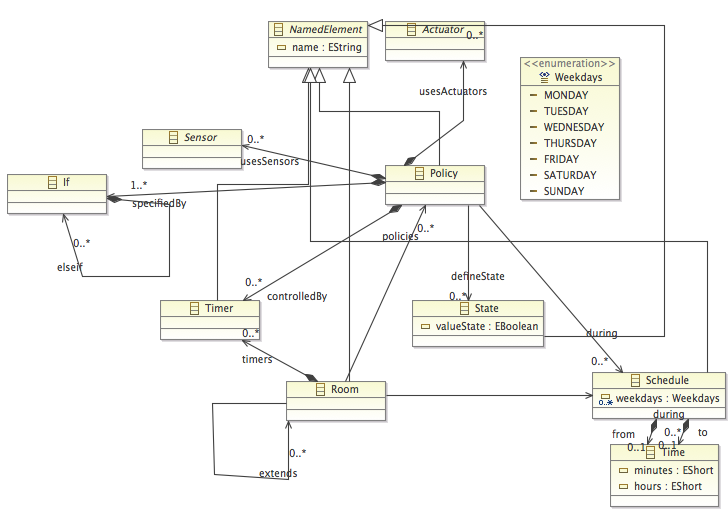
\includegraphics[scale=.5]{ecore-policy-definition.png}	
	\caption{The meta-model related to the \textit{policy definition}.}
	\label{fig:ecore-policy-definition}
\end{figure}

\subsection{Key Concepts}
During the analysis of the interviews, different meta-constructs were defined. It was evident that the \textit{three key concepts} listed below were needed in order to tailor core functionalities discovered.

\subsubsection{Time}\label{subsec:time}
Time has to be an integral part of the DSL, and not just related with the internal policy logic. Several interviewees mentioned concepts like weekdays, weekends, normal working hours, holidays, night, day, morning etc., which clearly shows that Time is necessary. We have extrapolated the need for Time in two different cases;
\begin{enumerate}
	\item Time conditional expressions\label{subsubsec:conditionalexpression}
are expressions used for determining the flow of a behavior. It is `if' statements that can react based on a built-in timer function (see fig.~\ref{fig:dsl-conditionalexpression}).

\begin{figure}[h]
  \centering
    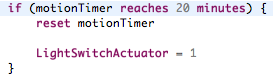
\includegraphics[scale=.5]{dsl-conditional-time-expression.png}
	\caption{An example of a \textit{time conditional expression} that evaluates to true if more than 20 minutes have elapsed.}
	\label{fig:dsl-conditionalexpression}
\end{figure}
\newpage
\item Schedules\label{subsubsec:schedules} are predefined types representing a timespan (see fig. \ref{fig:dsl-schedules}), which later can be attached to a specific behavior where action or no-action takes place. Note that by defining several \textit{schedules}, it is possible to make not only schedules that can overlap in time, but also policies that take over when other policies reach their end.

\begin{figure}
  \centering
  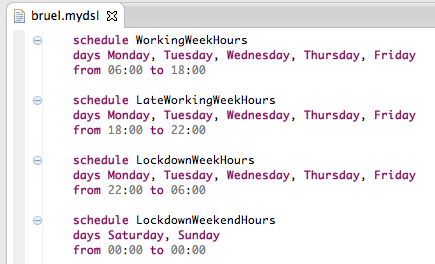
\includegraphics[scale=.5]{dsl-schedules.png}
  \caption{An example of a \textit{schedule}.}
  \label{fig:dsl-schedules}
\end{figure}
\end{enumerate}

\subsubsection{Policy}\label{subsec:policies}
Policies define the actual behavior, ie. adjustment of actuators, based on sensor input. In fig. \ref{fig:dsl-policy-definition}, when the \texttt{humiditySensor} value drops under 50, the \texttt{humidityAlarm} state is set to true. As long as the \texttt{humidityAlarm} is true, the \texttt{audioAlarmActuator} in the \texttt{janitorOffice} will sound every 15 seconds.

\begin{figure}[h]
  \centering
    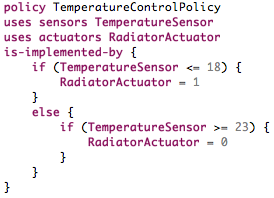
\includegraphics[scale=.5]{dsl-policy-definition.png} 
	\caption{An example of \textit{policy} using a single sensor type, and an actuator for a room instance.}
	\label{fig:dsl-policy-definition}
\end{figure}

\newpage
\subsubsection{Building specification}\label{subsec:buildingspecification}
Rooms and room types are part of the complete building specification, with terminology rooted in concepts revolving around buildings, ie. rooms, room types, floors, different sensors and actuators. \\

To avoid cluttering the DSL --- and confusing the user with an overwhelming amount of declarations of rooms, sensors and actuators --- we have designed \textit{room types} (fig. \ref{fig:room-types}) that declare static use of sensors and actuators. Rooms that does not fit into types, can still be internally defined by sensors and actuators on the instance level.

\begin{figure}
  \centering
    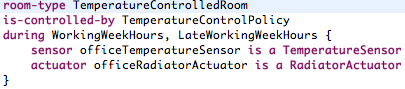
\includegraphics[scale=.5]{dsl-room-types.png}
	\caption{An example of \textit{room types}.}
	\label{fig:room-types}
\end{figure}

The \textit{building specification} (fig. \ref{fig:dsl-building-definition}) is the last piece of the BA puzzle --- it helps us analyze the the facilities that requires automation. Using this descriptive concept, we we are able to accurately define the real-world objects as \textit{buildings}, \textit{floors} and \textit{rooms} --- as well as implement policies for rooms in specific locations. 

\begin{figure}
  \centering
  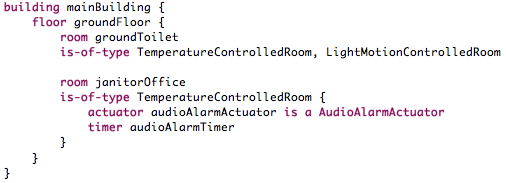
\includegraphics[scale=.5]{dsl-building-definition.png}  
  \caption{An example of \textit{building specification}. Note that the \textit{janitorOffice} inherits from a \textit{TemperatureControlledRoom} (which uses a \textit{TemperatureSensor} and a \textit{RadiatorActuator}) but also declares a \textit{AudioAlarmActuator} and a \textit{Timer} instance.}
  \label{fig:dsl-building-definition}
\end{figure}

All the sample DSL implementations as showns in the figures above, are possible by the fact that our grammar has a consistent forthcoming syntax and conceptual constructs. It has been tailored to fit the industry by making use of commonly used words in FM, which makes it clean, understandable and easy to use. (see \nameref{app:PedslXtext}).